\chapter{数据抽象和基本数据结构}

\section{概述}
数据抽象是允许我们将注意力放在数据结构的重要属性上的技术,而不管那些不重要的
未指明的概念。一个抽象数据类型(ADT)由申明的一系列数据结构和加在上面的一套操
作数据的操作组成。ADT的\emph{client},或者叫用户,调用这些操作来创建、销毁、
处理、询问(interrogate)抽象数据类型的\emph{对象}(或叫\emph{实例})。对于
这一点,一个\emph{client}是一些在ADT 外面定义的函数或过程。

本章描述了一种可以用来指明所需的抽象数据类型行为的技术,展示了如何将这种技术
使用到广泛使用的一些数据结构上,也回顾了在后面的算法开发中一些标准数据结构的重要
属性将其什么作用。

规范技术基于David Parnas的先驱工作(参见本章后面的注意和参考)。关键的思想叫
\emph{信息隐藏},或叫\emph{数据封装}。ADT模块含有私有数据,外部模块只能用定义
好的一些方法来存取这些私有数据。Parnas的目标是提供一种软件技术,使得大型工程
各部分都相互独立,但仍然正确的一起工作。

在算法设计和分析里面,ADT 还有其它的重要规则。主要设计可以使用ADT操作,而
不管操作是怎么实现的。我们可以在这个层次的算法设计完之后,再着手分析ADT操作在
算法中使用了多少次。有了这些信息,我们就可以优化ADT的实现,让执行最频繁的操作
开销最小。

换句话说,我们可以只使用ADT的逻辑属性就能考察一个算法的\emph{正确性},完全独立于
实现。但是\emph{性能分析}倚赖于实现。用ADT 涉及使得我们可以分开这两个概念。

\begin{figure*}[!t]
    \centering
    \begin{tikzpicture}[scale=0.8, place/.style={circle,draw, inner sep=0pt,minimum size=20mm},
        box/.style={rectangle,draw, inner sep=0pt,minimum size=16mm}]
        \node (pimer)  at ( 0,0) [place] {程序实现者};
        \node (a1imer) at ( 4,0) [place] {ADT1实现者};
        \node (a2imer)  at ( 8,0) [place] {ADT2实现者};
        \node [above] at (pimer.south) {ADT1 client};
        \node [above] at (a1imer.south) {ADT2 client};
        \node (ps)  at ( -2,4) [box] {程序规范};
        \node (a1s) at ( 2,4) [box] {ADT1规范};
        \node (a2s)  at ( 6,4) [box] {ADT2规范};
        \draw [->] (pimer.north) -- (ps.east);
        \draw [->] (pimer.north) -- (a1s.west);
        \draw [->] (a1imer.north) -- (a1s.east);
        \draw [->] (a1imer.north) -- (a2s.west);
        \draw [->] (a2imer.north) -- (a2s.east);

        \filldraw (1.8,-2) rectangle (2.2, 2);
        \filldraw (5.8,-2) rectangle (6.2, 2);
    \end{tikzpicture}
    \caption{ADT规范提供了client和实现者之间的界面。在这个例子中实现ADT1时使用了ADT2}
    \label{Fig:ExampleOfADT}
\end{figure*}

一种程序设计语言支持数据抽象的程度在于它是否允许程序员限制client对抽象数据类型
的存取;存取只能通过定义的方法,以及ADT 类的public部分。有private数据叫
\emph{数据封装}或叫\emph{信息隐藏}。这提供给程序员一个工具,程序员可以确保ADT
对象保持某种\emph{恒定}的状态。就是说,如果client唯一的存取ADT实例的方法是通过
一套比较小的由ADT 的接口定义的操作,则实现操作的程序员就可以(至少在理论上)
确保数据结构各个部分之间的关系符合ADT 的规范。图\ref{Fig:ExampleOfADT}展示了
这种情况。这些考虑解释了为什么在软件工程中ADT的重要。

我们选择Java作为实现算法的语言,主要是因为它简单,自然的支持数据抽象。在Java中
ADT作为一个类(但是,不是每一个类都是ADT;例如\ref{Sec:OrganizerClass}小节
的例子)程序可以创建\emph{类}的对象;这些对象是一个抽象数据类型的简单元素。

\section{ADT规格和设计技术}
ADT的\emph{规范}描述了操作有什么行为,这个信息对ADT的client十分重要。
就是说,规范应该避免引用私有实例域,因为client不知道私有实例域的存在。
规范描述了ADT公有部分--通常是操作和常量--之间的\emph{逻辑}关系。
(本章后面小节的例子中,将验证这个普遍性规律。)ADT操作(函数或过程)
在Java术语叫“方法(method)”。

这样设计ADT的一个显著的优点是,client可以在仅仅知道ADT规范的情况下
开发一个逻辑概念算法,client可以不管ADT的具体实现(甚至不管实现的
语言)。这也是本书使用ADT方法的主要动机。

\subsection{ADT设计规范}\label{Sec:ADTSpecification}
规范可以分为\emph{precondition}和\emph{postcondition}。一个特定
操作的\emph{precondition}是当操作被调用时假设为真的命题
\footnote{译者:即如果该命题不为真,则操作产生不可预知的结果,
比如假设传递进来的指针是非法的。}。
如果操作有参数,先决条件一个重要的功能是验证参数
\footnote{原文:If the operation has parameters it is important that
the preconditions be stated in terms of these parameters name for
clarity.}。在调用ADT的任何方法(静态方法、函数、过程)之前满足
preconditions是client的责任。一个特定方法的postcondition是client在
调用完方法返回之后认为已经为真的命题 \footnote{原文:If the operation
has parameters it is important that the preconditions be stated in
terms of these parameters
name}。另外,postcondition也叫做方法的目标(objectives)。

Java提供了一种特殊的用于class文档的注释格式,包含方法的preconditions
和postconditions。以“/**”开始的注释开始了一个javadoc注释。我们
在文本中使用\textbf{javadoc}注释约定来作为一个信号,表示这块注释表示
过程或一块代码的\emph{规范},否则注释是实现方式(即程序代码)的说明。

\subsubsection{What Goes into an ADT}
对于我们使用ADT的目的来说,ADT是一组相关的过程和函数,他们的规范
相互作用提供了一种特定的功能。我们采用最简单的视图,即只在ADT中包含
必要的操作;这些操作“需要知道”对象是如何实现的。因而ADT不是一个方便
的函数库;如果需要的话,一个库可以作为一个附加的类提供。

必要的操作可分为三个部分,\emph{构造函数},\emph{存取函数}和
\emph{处理函数}。销毁函数,销毁对象并释放对象占用存储空间的函数,
因为Java自动进行“垃圾收集”机制,析构函数不是必须的。垃圾收集定位
不引用的对象,回收他们的空间。

\begin{example}
ADT操作的类型

ADT操作的三种类型如下:

\begin{tabular}{ll}
    \emph{构造函数} & 创建新对象并返回对象的引用\\
    \emph{存取函数} & 返回对象的信息,但不改变它。\\
    \emph{处理函数} & 修改对象,但是不返回信息。\\
\end{tabular}

因而,在对象创建之后,一个操作可以修改对象,或者可以返回对象的信息,
但是不能同时进行两项操作。
\end{example}

注意ADT的构造函数不是Java中的构造函数,和其他类型的ADT操作一样,它是独立于
程序设计语言的。在Java中构造函数通过\textbf{new}关键字来调用,它使用的语法和其
他函数一样(非静态)。

因为前面提到的规则,存取函数不能修改对象的任何状态,ADT规范可能经常
以一种特殊的方式组织。对于存取函数,一般不需要给出它的postconditions。
此外,标注处理函数和构造函数的规范时,他们的效果必须尽量使用ADT存取函数
的术语来描述。有时规范需要标记许多操作的组合效果。乍一看,从ADT构造
函数和处理函数的事后条件找出一个存取函数的行为,似乎是不符合逻辑的。
然而,如果我们将存取函数看作一种对象的普通的“值”,那么则可以得到好的理解
:无论什么时候一个操作初始化或改变一个对象的状态,操作的postconditions
必须告诉我们(那一种都是相关的)对象新的普通的“值”。

在选择的一套ADT的操作里,比较重要的一点是保证有充足的存取函数来检查
所有操作的preconditions。这提供给client能力以检查操作的preconditions是否
满足。

对于实际的软件开发,有一个包含经常使用的ADT操作的库是十分方便的。库
与ADT的不同在于库里面的操作可以用ADT操作来实现;他们不需要知道对象是
如何实现的"look under the hood"。(当然,在有些时候,"look under the hood"
可以提供一个更快版本的库函数。)


\subsection{ADT设计技术}
一些我们在开发算法中用到的重要ADT的定义,将在本章后面的小节中给出。读者也
可以从例子中看到如何使用Java来定义和实现这些ADT。也可以轻易的领会到如何
用读者熟悉的其他程序设计语言来实现他们。

对于简单,非常标准的ADT,像链表,树,堆栈,和FIFO队列,设计中使用的
ADT可以最后才给出实现。有时其他ADT是标准ADT的client,直接将标准ADT作为
模块使用。

对于许多复杂非标准的ADT,比如字典,优先级队列,和联合查找(Union-Find),
ADT可以在设计使用他们的逻辑优点(比如分析正确性简单),但是在最后实现的
时候他们应该可以被方便的“展开”,实现算法使用到的特定情况。

本章剩下的部分展示了几种标准的数据结构和他们那相关联的抽象数据类型,
从简单到复杂。各种要给出的规范技术以他们出现的顺序排序。在本章中,除了链表,
其他ADT实现的方法都在练习中讨论。我们包括了一些简单Java代码的链表的例子,
作为引出其他解决方案的“砖头”\footnote{译者:抛砖引玉}。一般情况,实现都
在ADT的算法中讨论,所以实现可以简明的是对算法模式的使用。


\section{基本ADT-列表和树}
抽象数据类型列表和数是简单的,但是用途广泛的,他们的操作都能很容易的在
常数时间内实现。我们将为这些ADT指定一个构造器和一些存取函数,但是没有
处理函数。缺少处理函数使得规范非常简单。省略处理函数的另一个原因在
\ref{Sec:ListADT}节中解释。列表和树是最适合用递归来定义的。

\subsection{递归ADT}
\begin{figure*}[!t]
    \centering
    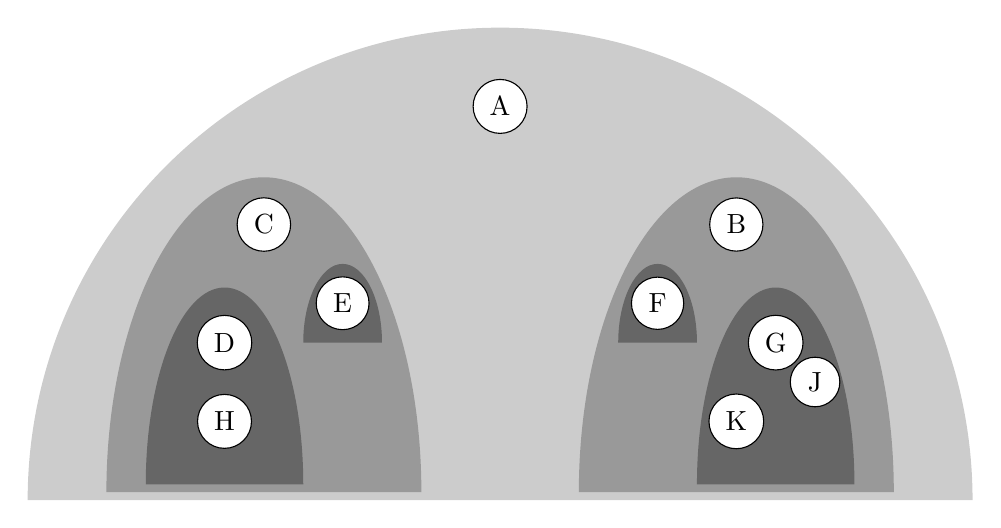
\begin{tikzpicture}[place/.style={circle,draw=black,fill=white}]
        \fill[black!20!white] (0, 0) arc(0:180: 6cm and 6cm);
        \fill[black!40!white] (-1, 0.1) arc(0:180: 2cm and 4cm);
        \fill[black!40!white] (-7, 0.1) arc(0:180: 2cm and 4cm);
        \fill[black!60!white] (-8.5, 0.2) arc(0:180: 1cm and 2.5cm);
        \fill[black!60!white] (-1.5, 0.2) arc(0:180: 1cm and 2.5cm);
        \fill[black!60!white] (-7.5, 2) arc(0:180: 0.5cm and 1cm);
        \fill[black!60!white] (-3.5, 2) arc(0:180: 0.5cm and 1cm);
        \node at(-6, 5)[place]{A};
        \node at(-3, 3.5)[place]{B};
        \node at(-9, 3.5)[place]{C};
        \node at(-9.5, 2)[place]{D};
        \node at(-9.5, 1)[place]{H};
        \node at(-8, 2.5)[place]{E};
        \node at(-4, 2.5)[place]{F};
        \node at(-2.5, 2)[place]{G};
        \node at(-2, 1.5)[place]{J};
        \node at(-3, 1)[place]{K};
    \end{tikzpicture}
    \caption{递归ADT中的对象必须是结构可以到达的所有部分,而不是只能直接存取得那一部分元素。}
    \label{Fig:ExampleOfRecursiveADT}
\end{figure*}

如果ADT的任何一个存取函数返回的都是自己的同类,则这个ADT是递归的。换句
话说,对象的有些部分(即存取函数返回的部分)和对象本身是同一类型。此时,
ADT常有一个拷贝构造函数,即构造函数的参数只有一个且类型为ADT的类型。
这样的ADT必须还有一个非递归的构造函数。但是,“非递归构造函数”常常简化
成一个常量(可以认为是一个没有参数的函数)。列表和树是最适合用递归来定义
的公用数据结构。我们将在\ref{Sec:ListADT}节到\ref{Sec:In-treeADT}节看到
他们的规范非常的简单和明了。

最好的理解递归数据结构类型对象的方法是将他看作一个结构,这个结构不仅包括
立即可存取得域,还包括只能通过ADT存取函数间接存取的域,存取函数返回一个
和ADT类型一样的对象。例如,在图\ref{Fig:ExampleOfADT}中,最好的理解根为A
的二叉树的方式是将它看作整个阴影的,尽管可以直接存取元素的只有根A。

\subsection{List ADT}\label{Sec:ListADT}
List\footnote{译者:List table翻译成汉语都是表,而list是一维,table是
二维故一律采用List英文单词。}是计算机科学中的基本
数据结构,在理论上和实践上都有重要的意义。许多算法以它开发,尽管可能
在程序设计语言中被叫做数组,list是数据结构中主要或者唯一的高效率版本。
程序设计语言Lisp是原有的将表作为唯一数据结构的程序设计语言。Lisp是“list
processing”(list处理)的缩写。许多其他程序设计语言,ML和Prolog将list
合并成了一种内建特性。这里说得表ADT类似于这些程序设计语言提供的list,
操作的名字采用Common Lisp的名字。

本文中的术语\emph{list}总是指数据结构内容中叫做\emph{链表linked
list}的东西。(对于一般的不指定数据结构的有序集合,我们使用术语
\emph{序列}。)短的术语\emph{list}是更合适的ADT的名字,因为没有术语
“link”出现在ADT的规范中;如果实现中使用了“link”,list的clients不关心
这个事实。

算法,特别是基于图的算法最常用到的list的类型就是整数list。因此,本节中
使用这种表做说明。

\textit{Java语法提示:}有经验的Java用户将尝试定义IntList以及其他特定元素
的list,作为一个非常通用List的子类。我们不需要这个做法,因为当元素是
原生类型时它带来很大的复杂性,而且它使得在继续后面的章节前必须清楚的
了解继承。这个主题于学习算法的关系不大。有很多关于Java语言的文章深入
讨论这个问题。

\begin{figure*}[!t]
\colorbox[rgb]{0.9, 0.9, 0.9}{IntList cons(int newElement, IntList oldList)}

\emph{preconditions:}无

\emph{postconditions:}如果x= cons(newElement, oldList), 则:
\begin{enumerate}
\item x引用一个新创建的对象;
\item $x\neq nil$
\item first(x)= newElement;
\item rest(x)=oldList
\end{enumerate}

\colorbox[rgb]{0.9, 0.9, 0.9}{int first(IntList aList)}

\emph{preconditions:}$aList \neq nil$

\colorbox[rgb]{0.9, 0.9, 0.9}{IntList rest(IntList aList)}

\emph{preconditions:}$aList \neq nil$

\colorbox[rgb]{0.9, 0.9, 0.9}{IntList nil}

表示空表的常量。

    \caption{IntList ADT的规范。函数cons是构造函数;first和rest是存取函数。
    List ADT是类似的,只是所有的int替换成Object,所有的IntList替换成List。
    其他类型元素的转换类似。}
    \label{Fig:ListADTSpecification}
\end{figure*}

IntListADT的规范在图\ref{Fig:ListADTSpecification}中展示。就像标题中指出的,将
list转换成其他类型是简单明了的。这些注释适用于代码,就像规范语句一样。在多个类中
使用cons、first、rest和nil不会引起混乱,因为语言要求用IntList.cons 来
访问在IntList类中的版本。

过程头,套在阴影中的部分,展示了Java或C语法中函数或过程的类型签名(申明)。
每一个参数都以其类型开始。因此cons的第一个参数是int,第二个参数是IntList。
在过程名字之前出现的类型或类的名字是返回类型。

规范其他的部分就是preconditions和postconditions。不需要将参数的类型必须
符合规定放到preconditions中去,因为这已经在原型中给出。于\ref{Sec:ADTSpecification}
节中的方法学一致,存取函数first和rest的行为,在cons的postconditions下描述。

回想一下List ADT的简单性是有价值的。当你停止考虑这个问题,这甚至是有趣的,
每一个可计算的函数都可以使用表作为唯一的数据结构\footnote{译者:图灵机的模型}。
有一个常量表示空的表,有一个函数(它的标准名字叫cons,所以我们采用这个名字)
通过将一个新元素放到原有表(这个表可能是空表)的前面来构造表。其他函数简单
的返回表(非空的)的信息。第一个元素是什么?表中其他元素是什么?很显然表的
所有操作都能在常数时间内完成。(我们假定为新对象分配内存只需要常数时间,
这是一个公共假设。)

\begin{figure*}[!t]
\begin{lstlisting}[language={Java},keywordstyle=\color{blue!70}, commentstyle=\color{red!50!green!50!blue!50}]
    import java.lang.*;
    public class IntList{
        int element;
        IntList next;

        /** `\color[rgb]{0.5, 0.5, 0.5}{常量nil表示空的表.}`*/
        public static final IntList nil= null;
        /** preconditions: `\color[rgb]{0.5, 0.5, 0.5}{L非nil.}`
            `\color[rgb]{0.5, 0.5, 0.5}{返回值:L的第一个元素.}`*/
        public static int first(IntList L){
            return L.element;
        }
        /** preconditions: `\color[rgb]{0.5, 0.5, 0.5}{L非nil.}`
            `\color[rgb]{0.5, 0.5, 0.5}{返回值:除了第一个元素以外,L其他元素构成的表.}`*/
        public static IntList rest(IntList L){
            return L.next;
        }
        /** preconditions: `\color[rgb]{0.5, 0.5, 0.5}{无}`
            *postconditions: `\color[rgb]{0.5, 0.5, 0.5}{令newL作为cons的返回值.}`
            *`\color[rgb]{0.5, 0.5, 0.5}{则:newL引用一个新的对象,newL非nil,}`
            *first(newL)= newElement,
            *rest(newL)= oldList. */
        public static IntList cons
            (int newElement, Intlist oldList){
            List newL = new IntList();
            newL.elemnet =newElement;
            newL.next =oldList;
            return newL;
        }
    }
\end{lstlisting}
    \caption{IntList ADT的一个Java类的典型实现。每一个有一个私有实例域
            element和next;公共域nil由于关键字final成为了常量;类剩下的
            部分是方法。Javadoc工具将"/**…*/" 形式的注释和跟在注释后面
            的程序元素关联起来,生成Web浏览器格式的文档。}
    \label{Fig:ImplementationOfRecursiveADT}
\end{figure*}

不需要改变ADT client的代码,IntList的规范可以以许多方式实现。图
\ref{Fig:ImplementationOfRecursiveADT}展示了一种典型的(也是最小的)实现。注意
这个实现没有对first和rest的preconditions做安全的测试。检查任何要调用函数
preconditions的安全性是调用者的责任。

为了软件工程的需要我们可能想创建一个叫IntListLib的类(这个类没有指定
构造函数。)这个库中可能需要包括length、copy、equals、reverse、sum、
max和min。

\textit{Java语言提示:}从调试的角度来看,包含Java error和exception特性
是很有帮助的,但是这使得写一整套ADT和ADT的clients的规范变得复杂。我们一直
采用的文字接近于解决问题的精练算法代码。我们提醒读者,将经常建议嵌入
软件工程方面的考虑。

\subsubsection{部分重建和非破坏性操作(Nondestructive Operations)}

\begin{figure*}[!t]
\centering
    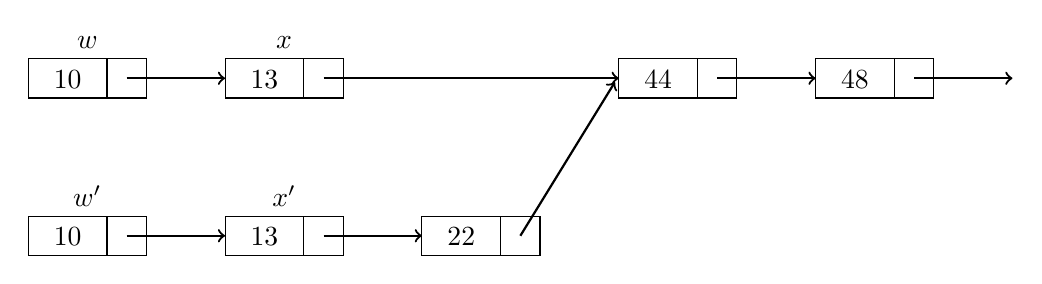
\begin{tikzpicture}
        \foreach \x in {0, 2.5, 5}
            \draw(\x+0, 0) rectangle (\x+1.5,0.5);
        \foreach \x in {0, 2.5, 5}
            \draw(\x+1, 0) -- (\x+1, 0.5);
        \foreach \x in {0, 2.5, 7.5, 10}
            \draw(\x+0, 2) rectangle (\x+1.5,2+0.5);
        \foreach \x in {0, 2.5, 7.5, 10}
            \draw(\x+1, 2) -- (\x+1, 2+0.5);

        \draw(0.75, 0.5) node[above]{$w'$};
        \draw(0.75+ 2.5, 0.5) node[above]{$x'$};
        \draw(0.75, 2+0.5) node[above]{$w$};
        \draw(0.75+ 2.5, 2+0.5) node[above]{$x$};

        \draw(0.5, 0) node[above]{10};
        \draw(0.5+ 2.5, 0) node[above]{13};
        \draw(0.5+ 5, 0) node[above]{22};

        \draw(0.5, 2) node[above]{10};
        \draw(0.5+ 2.5, 2) node[above]{13};
        \draw(0.5+ 7.5, 2) node[above]{44};
        \draw(0.5+ 10, 2) node[above]{48};

        \foreach \x in{1.25, 1.25+7.5, 1.25+ 10}
            \draw[->, thick](\x, 2.25)--(\x+1.25, 2.25);
        \foreach \x in{1.25, 1.25+2.5}
            \draw[->, thick](\x, 0.25)--(\x+1.25, 0.25);
        \draw[->, thick](1.25+2.5, 2.25)--(1.25+6.25, 2.25);
        \draw[->, thick](1.25+5, 0.25)--(1.25+6.25-0.05, 2.25-0.05) ;

    \end{tikzpicture}
    \caption{部分重建技术将22插入到顺序表10、13、44、48中。}
    \label{Fig:NonDestructiveOperations}
\end{figure*}

认真的读者可能想知道在IntList ADT的制度下我们如何\emph{修改}一个表。
答案很简单:我们不修改!这里没有\emph{处理过程}。这个ADT被称为非破坏性的
原因之一就是:一旦一个对象被创建,它就不能被修改。(术语\emph{不可修改的}
(\emph{immutable}) 也是这个含义。)为了更新一个list这里有三个选择:
\begin{enumerate}
\item 在一个面向对象语言中,比如Java,定义一个IntList类的派生类,在
        其中增加修改的功能(使得派生类是一个破坏性的或可修改)或者
\item 修改IntList本身,增加修改的功能(使其是一个\emph{破坏性的}或
        \emph{可修改})或者
\item 离开IntList本来的定义。为了完成修改,局部重建原来的表,产生一个
        新表,将表变量重新\emph{引用}新的表而代替原来的。
\end{enumerate}
局部重建的思想在图\ref{Fig:NonDestructiveOperations}中表示。目标是在
list中顶部标记为$w$的对象开始的表中,在已存在的元素13和44之间插入一个新元素22。
(按前面递归ADT的讨论,我们将$w$看作整个表,而不仅是第一个元素。)
在插入点之前,重建了包含元素10和13的的部分表,就像在图的下部展示的
一样。当然,为新元素22创建一个新的对象。但是新对象$x'$,包含一个新的13的
拷贝,$w'$包含一个新的10的拷贝也被创建了。对象$x$和$w$被完整的保留了。

一般情况下,部分重建意味着对于任何对象x,有一个域是我们要修改的,我们
创建一个新的对象$x'$,其他域都是一样的值,给需要修改的域一个新的值。$x$ $x'$所
引用的对象都不需要改变,这就是为什么重建是局部的。但是现在,如果也不能
修改的对象w引用x,我们想修改的效果也影响$w$,我们需要从$w$创建$w'$(除了$w'$引用
$x'$而不是$x$以外,其他都一样)来进行递归重建。就像我们在下一个例子中看到的,
定位$w$没有麻烦,因为我们仍然使用$w$来定位$x$,使用$w$来调用函数的地方仍是活的。
因此在创建$x'$的函数调用返回之后,我们回到了$w$是一个已知量的环境中。

\begin{figure*}[!t]
\begin{lstlisting}[language={Java},keywordstyle=\color{blue!70}, commentstyle=\color{red!50!green!50!blue!50}]
    /** `\color[rgb]{0.5, 0.5, 0.5}{preconditions: oldList是升序的。}`
    *   `\color[rgb]{0.5, 0.5, 0.5}{返回: 升序的新表,由newElement和oldList其他元素组成}`
    */
    public static IntList insertl
            (int newElement, IntList oldList){
        IntList newList;
        if(oldList == IntList.nil )
            newList = IntList.cons( newElement, oldList);
        else{
            int oldFirst= IntList.first(oldList);
            if(newElement <= oldFirst)
                // `\color[rgb]{0.5, 0.5, 0.5}{newElement 属于oldList的前面}`
                newList= IntList.cons
                        (newElement, oldList);
            else{
                IntList oldRest= IntList.rest(oldList);
                IntList newRest=
                    insertl(newElement, oldRest);

                // `\color[rgb]{0.5, 0.5, 0.5}{局部重建}`
                newList =IntList.cons(oldFirst, newRest);
            }
        }
        return newList;
    }
\end{lstlisting}

    \caption{在有序表中插入整数的函数(或Java方法),采用局部重建技术。
                注意,使用IntList类的成员时使用了完全名字。这是必须的
                因为insertl不在类中。}
    \label{Fig:PartialRebuild}
\end{figure*}

\begin{example}
通过局部重建在一个有序表中插入

图\ref{Fig:PartialRebuild}展示的Java代码通过局部重建的方法在一个已存在
的有序表中插入整数。在所有的递归开始之前,我们首先对一个基本事实进行检查:
\textbf{oldList}是空的吗?注意,空表是有序的!之后要检查的是另一个基本事实:
一个新元素可以简单的插入到oldList的前面吗?这两种情况下,\textbf{oldList}都
不需要修改,我们直接用\textbf{cons}在它前面插入一个新元素。

如果不是上面这两种情况,就要做一个递归函数,其返回一个重建的表(存储在
newRest),新元素在表适当的位置。现在我们的任务是在newRest的“前面”包含
oldList。既然我们不能修改对象oldList,我们通过调用cons创建新对象(存储在newList)
来“重建”。注意在这个递归过程中newList和oldList有相同的第一个元素。但是
rest(newList)与rest(oldList)不同,rest(newList)在合适的地方包含newElement。

这个过程是普通搜索例程的一个例子(参见定义\ref{Def:GeneralSearch})。我们在
包含元素的表的前面搜索一个较大的关键字的元素。“失败”事件是遇到空表,因为
显然没有更大的元素了。“成功”事件是在测试的表中第一个元素更大。如果这个两个
事件都没有发生,我们“继续搜索”剩下的表。每一个没有成功的搜索步骤都会发生一次
重建操作。

在调试和证明正确性的方面,局部变量的频繁使用。注意局部变量可以定义在“inner blocks”
中而不一定非要在函数的开始。另外注意,整个例子代码中。局部变量在每个函数调用
中只赋值一次;赋值一次是习惯,之后又用其他值改变会使得正确性问题变的复杂。
这个主题在\ref{Sec:WhatIsTheProof}节中做更深的讨论。

考虑图\ref{Fig:NonDestructiveOperations}的例子,将22插入到包含10,13,44,48
的表。初始表是$w$,10是第一个元素,$x$是剩下的表。既然22>10,22必须插入到$x$
之中,创建新表$x'$。第一次递归调用IntList.insert。22>13,第二次递归调用开始,
这次调用创建并返回一个新对象的引用,这个对象以22作为第一个元素。第一个元素
是44和48的对象不需要重建。

回到第一次递归调用,新对象$x'$被创建了,它的rest是刚返回的表,这个表的第一个
元素是22而且first从$x$拷贝。这个新对象 被返回到第一次调用(当然是它的引用被
返回了),它将$w$当作初始的表。初始调用创建$w'$,它的rest是$x'$,它的first
从$w$拷贝,返回一个引用$w'$的引用,按顺序插入的操作就完成了。因此当我们回到
递归开始位置的时候,对象$x$和$w$是从$x$和$w$重建的。

现在插入完成了,整个程序还需要$w$吗?显然,这是一个List ADT无法回答的问题。
如果回答是“no”,整个程序将(most likely)包含任何$w$的引用,应为所有指向$w$
的域或变量都指向了$w'$。如果回答是“yes”,仍然有一个重要的$w$的引用在程序的
某个地方。众所周知实践中,程序员决定何时释放和回收存储单元是许多隐晦错误的
根源,但是一个自动的垃圾收集机制将把程序员解放出来。

\textit{Java语言提示:}再次请使用C++的读者注意,Java不允许程序员定义一个新
版本的“<=”,所以在代码转换到非数值类之前,“<=”运算符必须由一个方法调用
代替。Java(从1.2版本)开始提供一个Comparable接口来用于在一般意义上排序类,
具体参见附录A。

许多其他的ADT都可以以List ADT为基础实现。多数例子是一般树(\ref{Sec:TreeADT}节)
和堆栈(\ref{Sec:StackADT}节)。其他将需要一个List ADT作为可更新的列表,
比如in-trees(\ref{Sec:In-treeADT}节)和队列(\ref{Sec:QueueADT}节)。

\end{example}

\subsection{二叉树ADT}\label{Sec:BinaryTreeADT}
我们可以认为二叉树是一个最简单的非线性列表的一般形式;与线性表一个元素只有
一个后继元素不同,二叉树中每一个元素有两个分支到不同的元素。在算法中,
二叉树有非常多的应用。

\subsubsection{二叉树的定义和基本属性}
数学上,\emph{二叉树T}是元素的集合,元素称为节点,节点可以是空或满足下列性质:
\begin{enumerate}
    \item 有一个独一无二的节点\emph{r}称为\emph{根}。
    \item 其余的节点分支为两个子集,\emph{L}和\emph{R},两个都是一个二叉树。
            \emph{L}称为T的\emph{左子树},\emph{R}称为T的\emph{右子树}。
\end{enumerate}

\begin{figure*}[!t]
    \centering
    \subfloat[带节点标签]{
        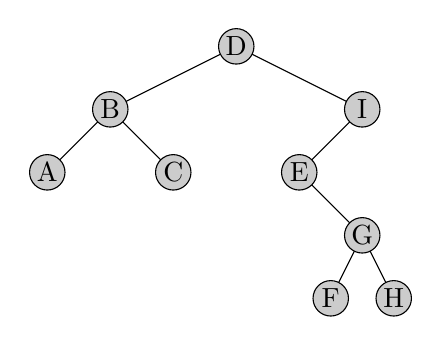
\begin{tikzpicture}[scale=0.8]
        \draw (4,3) -- (2, 2);
        \draw (4,3) -- (6, 2);
        \draw (2,2) -- (1, 1);
        \draw (2,2) -- (3, 1);
        \draw (6,2) -- (5, 1);
        \draw (5,1) -- (6, 0);
        \draw (6,0) -- (5.5, -1);
        \draw (6,0) -- (6.5, -1);

        \filldraw[fill=black!20!white] (4,3) circle(8pt) node{D};
        \filldraw[fill=black!20!white] (2, 2) circle (8pt) node{B};
        \filldraw[fill=black!20!white] (6, 2) circle (8pt) node{I};
        \filldraw[fill=black!20!white] (1,1) circle (8pt) node{A};
        \filldraw[fill=black!20!white] (3,1) circle (8pt) node{C};
        \filldraw[fill=black!20!white] (5,1) circle (8pt) node{E};
        \filldraw[fill=black!20!white] (6,0) circle (8pt) node{G};
        \filldraw[fill=black!20!white] (5.5,-1) circle (8pt) node{F};
        \filldraw[fill=black!20!white] (6.5,-1) circle (8pt) node{H};
        \end{tikzpicture}
        \label{Fig:BinaryTreeEx01_A}
    }
    \hfil
    \subfloat[完全]{
        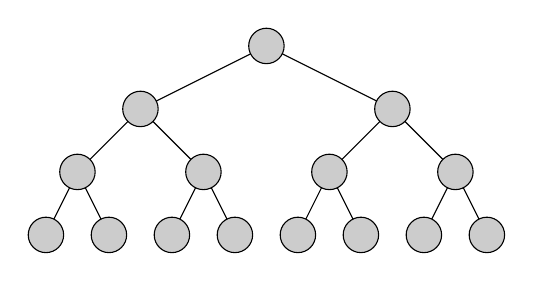
\begin{tikzpicture}[scale=0.8]
        \draw (4,3) -- (2, 2);
        \draw (4,3) -- (6, 2);
        \draw (2,2) -- (1, 1);
        \draw (2,2) -- (3, 1);
        \draw (6,2) -- (5, 1);
        \draw (6,2) -- (7, 1);
        \foreach \x in{1,3,5,7}
            \draw(\x ,1)--(\x+0.5, 0);
        \foreach \x in{1,3,5,7}
            \draw(\x ,1)--(\x-0.5, 0);

        \filldraw[fill=black!20!white] (4,3) circle(8pt) ;
        \filldraw[fill=black!20!white] (2, 2) circle (8pt) ;
        \filldraw[fill=black!20!white] (6, 2) circle (8pt);
        \foreach \x in{1, 3, 5, 7}
            \filldraw[fill=black!20!white] (\x,1) circle (8pt);
        \foreach \x in {0.5, 1.5, 2.5, 3.5, 4.5, 5.5, 6.5, 7.5}
            \filldraw[fill=black!20!white] (\x,0) circle (8pt);
        \end{tikzpicture}
        \label{Fig:BinaryTreeEx01_B}
    }
    \caption{二叉树}
    \label{Fig:BinaryTreeEx01}
\end{figure*}

二叉树在纸上通常以图\ref{Fig:BinaryTreeEx01}那样的图例来表示。如果节点
$\nu$是二叉树T的\emph{根},且节点$\omega$
是T的左(右)子树的根,则$\omega$叫做$\nu$的\emph{左(右)}孩子,
而$\nu$叫做$\omega$的\emph{parent};在图中从$\nu$到
$\omega$有一条直接的边。(边虽然没有箭头,但约定是向下的。)

树节点的度是它的非空子树的个数。度为0的节点是叶子。有正数度的节点称为
\emph{内节点(internal nodes)}。

根的深度是0,其他节点的深度是其双亲节点深度+1
\footnote{原注:小心,有的著作将根的深度定义为1}。一颗完全二叉树的所有
内节点的度是2,所有的叶子节点都在同一深度。图\ref{Fig:BinaryTreeEx01}右边
的树就是完全二叉树。

二叉树的\emph{高度}(有时候也叫做深度)是它的叶子最深的深度。任意二叉树节点
的\emph{高度}是以它为根的子树的深度。图\ref{Fig:BinaryTreeEx01_A}中,I的深度
是1,I的高度是3;D的深度是0,高度是4。

下面的事实在后面经常用到。证明他们很容易,在这里省略证明。

\begin{lemma}
深度为$d$的二叉树至多有$2^d$个节点。
\end{lemma}

\begin{lemma}
高度为$h$的二叉树至多有$2^{k+1}-1$个节点。
\end{lemma}

\begin{lemma}
有$n$个节点的二叉树其深度至少是$\lceil\lg(n+1)\rceil-1$。
\end{lemma}

\begin{figure*}[!t]
\colorbox[rgb]{0.9, 0.9, 0.9}{BinTree buildTree(Object newRoot, BinTree oldT, BinTree oldRT)}

\emph{preconditions:}无

\emph{postconditions:}如果 x=buildTree(newRoot, oldLT,oldRT), 则:
\begin{enumerate}
\item x引用一个新创建的对象;
\item $x\neq nil$
\item root(x)= newRoot;
\item leftSubTree(x)=oldLT
\item rightSubTree(x)=oldRT
\end{enumerate}

\colorbox[rgb]{0.9, 0.9, 0.9}{Object  root(BinTree t)}

\emph{preconditions:}$t \neq nil$

\colorbox[rgb]{0.9, 0.9, 0.9}{BinTree  leftSubtree(BinTree t)}

\emph{preconditions:}$t \neq nil$

\colorbox[rgb]{0.9, 0.9, 0.9}{BinTree  rightSubtree(BinTree t)}

\emph{preconditions:}$t \neq nil$

\colorbox[rgb]{0.9, 0.9, 0.9}{BinTree  nil}

表示空树的常量。

    \caption{BinTree ADT的规范。函数buildTree是构造函数;root,
            leftSubtree和rightSubtree是存取函数。类中比\textbf{Object}
            一般的节点的规范以类似的方法定义。}
    \label{Fig:BinaryTreeSpecification}
\end{figure*}

图\ref{Fig:BinaryTreeSpecification}给出了BinTree ADT的规范。这显然是\ref{Sec:ListADT}
节表ADT的类推。存取root的函数是List.first的类推;它存取立即有效的数据。当然,
List.rest在这里分成了两个存取函数,leftSubtree和rightSubtree,使得client可以
存取树剩下的部分。
\footnote{原注:这里的命名不是标准的,在其他地方使用“leftChild”和“rightChild”。
但是讲述ADT的章节中,最好是将整个树当成一个对象看待,而不是只考虑根节点。
在我们的术语中,左右孩子分别表示左子树和右子树的根。}


\subsubsection{二叉树的遍历}
\begin{figure*}[!t]
    \centering
    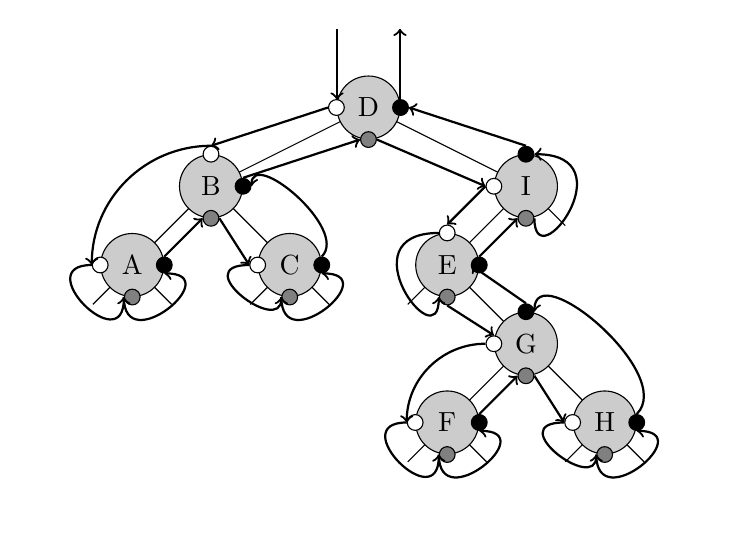
\begin{tikzpicture}[scale=1,
        place/.style={circle,draw, fill=black!20!white,inner sep=0pt,minimum size=8mm},
        lw/.style={circle,draw, fill=white, inner sep=0pt,minimum size=2mm},
        lg/.style={circle,draw, fill=gray, inner sep=0pt,minimum size=2mm},
        lb/.style={circle,draw, fill=black, inner sep=0pt,minimum size=2mm}]
        \foreach \x in {2,6}
            \draw (4,3) -- (\x, 2);
        \draw (2,2) -- (1, 1);
        \draw (2,2) -- (3, 1);
        \draw (6,2) -- (5, 1);
        \draw (5,1) -- (6, 0);
        \foreach \x in {1, 3}
            \draw (\x,1) -- (\x+0.5, 0.5);
        \foreach \x in {1, 3, 5}
            \draw (\x,1) -- (\x-0.5, 0.5);
        \foreach \x in {5, 7}
            \draw (\x,-1) -- (\x+0.5, -1.5);
        \foreach \x in {5, 7}
            \draw (\x,-1) -- (\x-0.5, -1.5);
        \draw (6,2 ) -- (6+0.5, 1.5);
        \draw (6,0) -- (5, -1);
        \draw (6,0) -- (7, -1);

        \node (D)  at (4,3) [place] {D};
        \node (Dw) at (D.west) [lw]{};
        \node (Db) at (D.east) [lb]{};
        \node (Dg) at (D.south) [lg]{};

        \node (B)  at (2,2) [place] {B};
        \node (Bw) at (B.north) [lw]{};
        \node (Bb) at (B.east) [lb]{};
        \node (Bg) at (B.south) [lg]{};

        \node (I)  at (6,2) [place] {I};
        \node (Iw) at (I.west) [lw]{};
        \node (Ib) at (I.north) [lb]{};
        \node (Ig) at (I.south) [lg]{};

        \node (A)  at (1,1) [place] {A};
        \node (Aw) at (A.west) [lw]{};
        \node (Ab) at (A.east) [lb]{};
        \node (Ag) at (A.south) [lg]{};

        \node (C)  at (3,1) [place] {C};
        \node (Cw) at (C.west) [lw]{};
        \node (Cb) at (C.east) [lb]{};
        \node (Cg) at (C.south) [lg]{};

        \node (E)  at (5,1) [place] {E};
        \node (Ew) at (E.north) [lw]{};
        \node (Eb) at (E.east) [lb]{};
        \node (Eg) at (E.south) [lg]{};

        \node (G)  at (6,0) [place] {G};
        \node (Gw) at (G.west) [lw]{};
        \node (Gb) at (G.north) [lb]{};
        \node (Gg) at (G.south) [lg]{};

        \node (F)  at (5,-1) [place] {F};
        \node (Fw) at (F.west) [lw]{};
        \node (Fb) at (F.east) [lb]{};
        \node (Fg) at (F.south) [lg]{};

        \node (H)  at (7,-1) [place] {H};
        \node (Hw) at (H.west) [lw]{};
        \node (Hb) at (H.east) [lb]{};
        \node (Hg) at (H.south) [lg]{};

        \draw [->, thick] (Dw.west) -- (Bw.north);
        \draw [->, thick] (Bw.north) to [out=180,in=90] (Aw.west);
        \draw [->, thick] (Aw.west)  .. controls +(left:8mm) and +(down:8mm) .. (Ag.west);
        \draw [->, thick] (Ag.west)  .. controls +(down:8mm) and +(right:8mm) .. (Ab.south);
        \draw [->, thick] (Ab.north)  -- (Bg.west);
        \draw [->, thick] (Bg.east)  -- (Cw.west);
        \draw [->, thick] (Cw.west)  .. controls +(left:8mm) and +(down:5mm) .. (Cg.west);
        \draw [->, thick] (Cg.west)  .. controls +(down:8mm) and +(right:8mm) .. (Cb.south);
        \draw [->, thick] (Cb.north) to [in=180,in=90]   (Bb.east);
        \draw [->, thick] (Bb.north)  -- (Dg.west);
        \draw [->, thick] (Dg.east)  -- (Iw.west);
        \draw [->, thick] (Iw.west)  -- (Ew.north);
        \draw [->, thick] (Ew.west)  .. controls +(left:12mm) and +(down:8mm) .. (Eg.west);
        \draw [->, thick] (Eg.south)  -- (Gw.north);
        \draw [->, thick] (Gw.west) to [out=180,in=90] (Fw.west);
        \draw [->, thick] (Fw.west)  .. controls +(left:8mm) and +(down:8mm) .. (Fg.west);
        \draw [->, thick] (Fg.west)  .. controls +(down:8mm) and +(right:8mm) .. (Fb.south);
        \draw [->, thick] (Fb.north)  -- (Gg.west);
        \draw [->, thick] (Gg.east)  -- (Hw.west);
        \draw [->, thick] (Hw.west)  .. controls +(left:8mm) and +(down:5mm) .. (Hg.west);
        \draw [->, thick] (Hg.west)  .. controls +(down:8mm) and +(right:8mm) .. (Hb.south);
        \draw [->, thick] (Hb.north) to [in=180,in=90]   (Gb.east);
        \draw [->, thick] (Gb.north)  -- (Eb.west);
        \draw [->, thick] (Eb.north)  -- (Ig.west);
        \draw [->, thick] (Ig.east) .. controls +(down:8mm) and +(right:12mm) ..    (Ib.east);
        \draw [->, thick] (Ib.north)  -- (Db.east);
        \draw[<-, thick] (4.4,4) --(4.4, 3.1);
        \draw[->, thick] (3.6,4) --(3.6, 3.1);
    \end{tikzpicture}
    \caption{二叉树遍历如同围绕树的旅行。}
    \label{Fig:BinaryTreeTraverse}
\end{figure*}
我们可以用图的方式表示二叉树的标准遍历,如同在树上进行从根开始的乘船旅行一样,
如图\ref{Fig:BinaryTreeTraverse}所示。我们将每一个节点想像成岛,每一个边是桥,
而桥太低以至船无法通过。为了使我们的想像总是正确,假设在没有子树的地方有桥墩
伸出。)小船从根节点开始沿着边航行,访问沿线的节点。节点第一次被访问(白色点),
叫做它的\emph{preorder time},它第二次被访问到(灰色点,从左孩子返回的那一次)
叫做\emph{inorder time},最后一次访问到(黑色的点,从右孩子返回的那一次)叫做
\emph{postorder time}。三次遍历可以用下面的递归过程优雅的表示:

\begin{figure}
\begin{lstlisting}[language={Java}, keywordstyle=\color{blue!70}, commentstyle=\color{red!50!green!50!blue!50}]
    void traverse(BinTree T)
    {   if(T is not empty)
        {   Preorder-process root(T);
            traverse(leftSubtree(T));
            Inorder-process root(T);
            traverse(rightSubtree(T));
            Postorder-process root(T);
        }
        return;
    }
\end{lstlisting}
\end{figure}
traverse的返回类型将随应用的不同而变化,它也可能需要额外的参数。前面的过程
展示了一个框架。

对于图\ref{Fig:BinaryTreeTraverse}中的二叉树,遍历树的顺序如下:

    Preorder(白点):  D B A C I E G F H

    Inorder(灰点):   A B C D E F G H I

    Postorder(黑点): A C B F H G E I D



\subsection{树ADT}\label{Sec:TreeADT}
\emph{一般的}树(更精确的说,\emph{一般的}out-tree)是一种带节点和有向边的
非空结构,有一个没有入边的节点称为\emph{根节点},它的其他节点都有且仅有一个
入边。更进一步说,就是根到每一个节点都有路径。每一个节点出边的数量没有限制。
\emph{森林}是独立树的集合。

一个节点的\emph{子树}由它能访问到的所有节点和它自己组成,节点是它\emph{子树}
的根。默认的每一个边都是从双亲到孩子的。如果节点$v$是节点$w$的双亲,则以$w$
为根的树称为以$v$为根的树的\emph{principal(主要)}子树。树的每一个首要子树
的节点都比树自己的节点要少。为每一个首要子树命名是不可行的,所以树ADT有时
比二叉树ADT要复杂。

对于一般的树,子树没有必要有顺序,而在二叉树中他们分为“左”和“右”。
(如果一般树的子树被认为是有顺序的,这种结构称为顺序树“ordered tree”。)
另一个与二叉树的区别是没有空的一般树。

\begin{figure*}[!t]
    \centering
    \subfloat[out-tree]{
        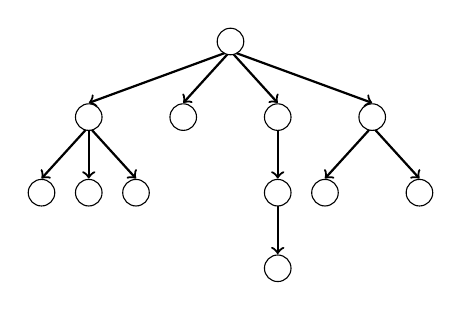
\begin{tikzpicture}[scale=1.2]
        \foreach \x in{1, 2, 3, 4}
            \draw[->, thick](2.5,2.3) -- (\x, 1.75) ;
        \foreach \x in{0.5, 1, 1.5}
            \draw[->, thick](1,1.5) -- (\x, 0.95) ;
        \foreach \x in{3.5, 4.5}
            \draw[->, thick](4,1.5) -- (\x, 0.95) ;
        \draw[->, thick](3,1.5) -- (3, 0.95) ;
        \draw[->, thick](3,0.95) -- (3, 0.15) ;

        \filldraw[fill=white] (2.5,2.4) circle(4pt) ;
        \foreach \x in{1, 2, 3, 4}
            \filldraw[fill=white] (\x, 1.6) circle(4pt) ;
        \foreach \x in{0.5,1, 1.5, 3, 3.5, 4.5}
            \filldraw[fill=white] (\x, 0.8) circle(4pt) ;
        \filldraw[fill=white] (3, 0) circle(4pt) ;
        \end{tikzpicture}
        \label{Fig:OutTreeAndInTree_A}
    }
    \hfil
    \subfloat[in-tree]{
        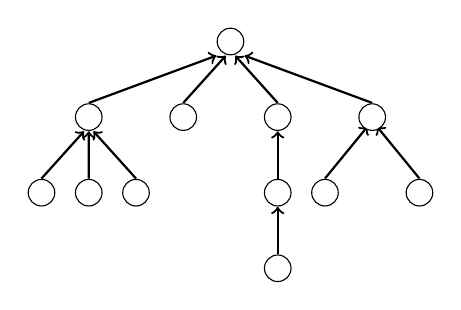
\begin{tikzpicture}[scale=1.2]
        \foreach \x in{1, 2, 3, 4}
            \draw[<-, thick]( 2.25+\x/10, 2.25) -- (\x, 1.75) ;
        \foreach \x in{0.5, 1, 1.5}
            \draw[<-, thick](0.9+\x/10, 1.45) -- (\x, 0.95) ;
        \foreach \x in{3.5, 4.5}
            \draw[<-, thick](3.6+\x/10,1.5) -- (\x, 0.95) ;
        \draw[<-, thick](3,1.45) -- (3, 0.95) ;
        \draw[<-, thick](3,0.65) -- (3, 0.15) ;

        \filldraw[fill=white] (2.5,2.4) circle(4pt) ;
        \foreach \x in{1, 2, 3, 4}
            \filldraw[fill=white] (\x, 1.6) circle(4pt) ;
        \foreach \x in{0.5,1, 1.5, 3, 3.5, 4.5}
            \filldraw[fill=white] (\x, 0.8) circle(4pt) ;
        \filldraw[fill=white] (3, 0) circle(4pt) ;
        \end{tikzpicture}
        \label{Fig:OutTreeAndInTree_B}
    }
    \caption{一般的out-tree和对应的in-tree。}
    \label{Fig:OutTreeAndInTree}
\end{figure*}

如果所有的边都是朝向根而不是离开根,这种结构称为\emph{in-tree},所有的边都是
从孩子到双亲(图\ref{Fig:OutTreeAndInTree})。对于这种不同的树有不同数据结构
和操作,将在\ref{Sec:In-treeADT}小节讨论。

\begin{figure*}[!t]
\colorbox[rgb]{0.9, 0.9, 0.9}{Tree buildTree(Object newRoot, TreeList oldTrees)}

\emph{preconditions:}无

\emph{postconditions:}如果 x=buildTree(newRoot, oldTrees), 则:
\begin{enumerate}
\item x引用一个新创建的对象;
\item $x\neq nil$
\item root(x)= newRoot;
\item subtrees(x)=oldTress;
\end{enumerate}

\colorbox[rgb]{0.9, 0.9, 0.9}{Object root(Tree t)}

\emph{preconditions:}无

\colorbox[rgb]{0.9, 0.9, 0.9}{TreeList subtrees(Tree t)}

\emph{preconditions:}无

TreeList ADT是一个类似IntList的表,基本元素是Tree。原型如下:

    TreeList cons(Tree t, TreeList rSiblings)

    Tree first(TreeList siblings)

    TreeList rest(TreeList siblings)

    TreeList nil

    \caption{树ADT的规范。类中比\textbf{Object}一般的节点的规范以类似的方法定义。}
    \label{Fig:TreeSpecification}
\end{figure*}

树ADT(最小的操作集合)由图\ref{Fig:TreeSpecification}的规范描述。与二叉树类似
的就省略了。与二叉树不同的是,二叉树的两个子树都有名字,在树中,我们没有定义
主要子树的数量,所以List是描述这些子树的自然选择。除非树是顺序树,否则是不
关心列表的顺序的,子树可以看成是一个集合而不是序列。

第一个主要子树,叫做$t_0$,\emph{最左子树};$t_0$的root称为\emph{最左孩子}。对于
任意主要子树,$t_i$,序列中的下一个主要子树是$t_{i+1}$,如果$t_{i+1}$存在,称为
$t_i$的\emph{右表兄子树}。参见图\ref{Fig:StructureOfTree}例子。尽管这里使用这样
的术语,我们重申表中子树的相关顺序对于抽象的树是没有意义的,仅仅因为我们使用
List来存放子树。ADT的构造函数buildTree合并一个根节点和树的list,来创建更大的树。

\begin{figure*}[!t]
    \centering
    \subfloat[逻辑结构]{
        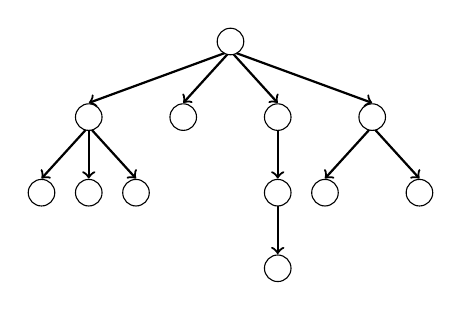
\begin{tikzpicture}[scale=1.2]
        \foreach \x in{1, 2, 3, 4}
            \draw[->, thick](2.5,2.3) -- (\x, 1.75) ;
        \foreach \x in{0.5, 1, 1.5}
            \draw[->, thick](1,1.5) -- (\x, 0.95) ;
        \foreach \x in{3.5, 4.5}
            \draw[->, thick](4,1.5) -- (\x, 0.95) ;
        \draw[->, thick](3,1.5) -- (3, 0.95) ;
        \draw[->, thick](3,0.95) -- (3, 0.15) ;

        \filldraw[fill=white] (2.5,2.4) circle(4pt) ;
        \foreach \x in{1, 2, 3, 4}
            \filldraw[fill=white] (\x, 1.6) circle(4pt) ;
        \foreach \x in{0.5,1, 1.5, 3, 3.5, 4.5}
            \filldraw[fill=white] (\x, 0.8) circle(4pt) ;
        \filldraw[fill=white] (3, 0) circle(4pt) ;
        \end{tikzpicture}
        \label{Fig:StructureOfTree_A}
    }
    \hfil
    \subfloat[基于表的结构]{
        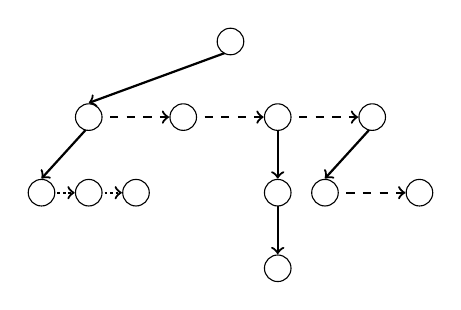
\begin{tikzpicture}[scale=1.2]
        \draw[->, thick](2.5, 2.3)--(1, 1.75);
        \draw[->, thick,dash pattern=on 3pt off 3pt](1.05,1.6) -- (1.85, 1.6);
        \draw[->, thick,dash pattern=on 3pt off 3pt](2.05,1.6) -- (2.85, 1.6);
        \draw[->, thick,dash pattern=on 3pt off 3pt](3.05,1.6) -- (3.85, 1.6);
        \draw[->, thick,dash pattern=on 1pt off 1pt](0.55,0.8) -- (0.85, 0.8);
        \draw[->, thick,dash pattern=on 1pt off 1pt](1.05,0.8) -- (1.35, 0.8);
        \draw[->, thick,dash pattern=on 3pt off 3pt](3.55,0.8) -- (4.35, 0.8);
        \draw[->, thick](1,1.5) -- (0.5, 0.95);
        \draw[->, thick](4,1.5) -- (3.5, 0.95);
        \draw[->, thick](3,1.5) -- (3, 0.95) ;
        \draw[->, thick](3,0.95) -- (3, 0.15) ;

        \filldraw[fill=white] (2.5,2.4) circle(4pt) ;
        \foreach \x in{1, 2, 3, 4}
            \filldraw[fill=white] (\x, 1.6) circle(4pt) ;
        \foreach \x in{0.5,1, 1.5, 3, 3.5, 4.5}
            \filldraw[fill=white] (\x, 0.8) circle(4pt) ;
        \filldraw[fill=white] (3, 0) circle(4pt) ;
        \end{tikzpicture}
    }
    \caption{(a)是一般out-tree的逻辑或概念上的结构,(b)则是相应的以list存储
            子树的结构:朝下的实线箭头到最左边的子树,虚线箭头指向右表兄子树。}
    \label{Fig:StructureOfTree}
\end{figure*}

\emph{Java语言提示:}为了在Java中定义这样的内部相关ADTs而且具有理想的看见性控制,
必须使用Java的package。两个文件必须在同一目录中,必须命名为Tree.java和TreeList.java。
细节不是困难,但是他们属于本书的范围。将client和ADTs放在相同的目录下,以
避免需要处理包的细节。

\begin{figure*}[!t]
    \centering
    \begin{lstlisting}[language={Java}, keywordstyle=\color{blue!70}, commentstyle=\color{red!50!green!50!blue!50}]
        void traverse(Tree T)
        {   TreeList remainSubs;
            Preorder-process Tree.root(T);
            remainSubTrees= Tree.subtrees(T);
            while(remainSubtrees  TreeList.nil)
            {   Tree subtree=
                    TreeList.first(remainSubtrees);
                traverse(subtree);
                Inorder-process Tree.root(T) and subtree;
                remainSubtrees=
                    TreeList.rest(remainSubtrees);
            }
            Postorder-process Tree.root(T);
            return;
        }
    \end{lstlisting}
    \caption{树的遍历框架}
    \label{Fig:FrameworkOfTraverseTree}
\end{figure*}

树的遍历可以通过对二叉树遍历(参见\ref{Sec:BinaryTreeADT}小节)进行逻辑扩展来
表示,图\ref{Fig:FrameworkOfTraverseTree}展示了一个框架。子树在一个while循环
中遍历,因为子树的数量是不定的,而且有不能确定数量的中序次数。(这里都使用了
类全名,因为牵涉到两个类。)遍历的返回类型将是和具体应用相关的,它也可能需
要额外的参数。图\ref{Fig:FrameworkOfTraverseTree}展示了一个通用的框架。


\subsection{In-tree ADT}\label{Sec:In-treeADT}
\emph{It is a wise father that knows his own child.}

\indent\indent\indent    - Shakespeare, The Merchant of Venice

通常,对于树的存取模式都是从根到叶子,一般描述为向下的方向。但是有时需要从
叶子向根访问(朝上,比如图\ref{Fig:OutTreeAndInTree_B}),而且不需要向下访问。
一个in-tree是只提供这种访问方式的树:节点不“知道”它的孩子。

in-tree树的一个重要概念是\emph{祖先(ancestor)},可以由下面的递归形式定义。

\begin{definition}


节点$v$是它自己的祖先。如果$p$是$v$的双亲,则每一个$p$的祖先都是$v$的祖先。
祖先的反转是\emph{后代(descendant)}。
\end{definition}

在in-tree中,一个节点可以访问它的祖先,但是不能访问它的后代。不像普通
的\emph{Tree ADT},在Tree ADT中对象是整个树;在in-tree的一个对象是一个节点
和它的祖先,所以类的名字是\textbf{InTreeNode},ADT的构造函数是\textbf{makeNode}。

令$v$是类InTreeNode的一个对象。我们遍历树需要那些存取函数呢?首先需要的存取函数
是isRoot(v),一个布尔函数,当$v$没有双亲时返回\textbf{true}。其次需要的存取函数
是parent(v),它的一个precondition是isRoot(v)返回\textbf{false}。换句话说,只要
isRoot(v)是\textbf{true},则调用parent(v)是错误的。

\begin{figure*}[!t]
\colorbox[rgb]{0.9, 0.9, 0.9}{InTreeNode makeNode(int d)}

\emph{preconditions:}无

\emph{postconditions:}如果x=makeNode(d)则:
\begin{enumerate}
\item x引用一个新创建的对象;
\item nodeData=d;
\item isRoot(x)=true;
\end{enumerate}

\colorbox[rgb]{0.9, 0.9, 0.9}{boolean isRoot(InTreeNode v)}

\emph{preconditions:}无

\colorbox[rgb]{0.9, 0.9, 0.9}{InTreeNode parent(InTreeNode v)}

\emph{preconditions:}isRoot(v)=false.

\colorbox[rgb]{0.9, 0.9, 0.9}{int nodeData(InTreeNode v)}

\emph{preconditions:}无.

\colorbox[rgb]{0.9, 0.9, 0.9}{void setParent(InTreeNode v, InTreeNode p)}

\emph{preconditions:}Node v不是p的祖先。

\emph{postconditions:}
\begin{enumerate}
\item nodeData(v)保持不变;
\item parent(v)=p;
\item isRoot(v)=false;
\end{enumerate}

\colorbox[rgb]{0.9, 0.9, 0.9}{setNodeData(InTreeNode v, int d)}

\emph{preconditions:}无。

\emph{postconditions:}
\begin{enumerate}
\item nodeData(v)保持不变;
\item parent(v)保持不变;
\item isRoot(v)保持不变;
\end{enumerate}

    \caption{InTreeNode ADT的规范。函数makeNode是构造函数;isRoot,
            parent,nodeData是存取函数;setParent和setNodeData是处理函数。
            节点数据是不同于\textbf{int}的其他类时,规范类似。}
    \label{Fig:InTreeADTSpecification}
\end{figure*}

图\ref{Fig:InTreeADTSpecification}包含了InTreeNode ADT的规范。当一个节点是
由makeNode构造的,它是树的唯一节点,所以isRoot是\textbf{true}。显然我们需要
构造更大树的方法。不像其他简单ADT,这里使用了一个\emph{处理函数}来获得这个
功能。处理函数的返回类型总是\textbf{void};他们不返回值。这个处理函数是
setParent(v,p),它将$p$设置成$v$的双亲。有一个precondition是$v$必须不是$p$的
祖先(否则会创建一个环)。它的postconditions是isRoot(v)是false,以及
parent(v)返回p。

实际应用,通常需要在节点保留一种类型数据。既然in-tree结构没有其他的分支,
我们能定义简单的一对操作,setNodeData和nodeData,来允许client存储获得这样的
数据。尽管节点数据依赖于具体的应用可能有不同的类型,我们按int定义,因为int最
常见。例如,尽管一个节点不知道它的后代,但是可以保存一个每个节点到底有多少
后代的记录(练习2.12)。

In-tree常嵌在其他的数据结构中,而不是作为一个独立的ADT。这几乎是必须的,因为
从任何一个in-tree的节点出发都不能访问整个树。我们将在图的最小生成树,和最短路径
算法中遇到in-tree,实现联合查找ADT时也要用到。联合查找ADT在各种算法中用到,包括
一种最小生成森林算法。

\section{堆栈和队列}
堆栈和队列说明了抽象数据类型规范下一个级别的复杂性。他们的ADT包括
操作过程,所以在一类对象可以改变他们的“状态”。现在规范需要描述什么样的
状态改变可以发生。然而,这些通用ADT上的所有的操作都可以在常数时间内完成,
没有太多的难度。有时我们需要保存任务的轨迹,而一个任务可能产生不可预知数量
的其他任务,堆栈和队列是一个好的选择。


\subsection{堆栈ADT}\label{Sec:StackADT}

\begin{figure*}[!t]
\colorbox[rgb]{0.9, 0.9, 0.9}{Stack create()}

\emph{preconditions:}无

\emph{postconditions:}如果s=create()则:
\begin{enumerate}
\item s引用一个新创建的对象;
\item isEmpty(s)=true;
\end{enumerate}

\colorbox[rgb]{0.9, 0.9, 0.9}{boolean isEmpty(Stack s)}

\emph{preconditions:}无

\colorbox[rgb]{0.9, 0.9, 0.9}{Object top(Stack s)}

\emph{preconditions:}isEmpty(s) =false.

\colorbox[rgb]{0.9, 0.9, 0.9}{void push(Stack s, Object e)}

\emph{preconditions:}无

\emph{postconditions:}
\begin{enumerate}
\item top(s) =e;
\item isEmpty(s)= false;
\end{enumerate}

\colorbox[rgb]{0.9, 0.9, 0.9}{void pop(Stack s)}

\emph{preconditions:}isEmpty(s) =false.

\emph{Postconditions:}参见下面的解释。

\emph{注解:}在create之后,任何合法的push和pop操作(例如累计起来,pop的数量
绝没有push多)的序列会产生一个有同样状态的堆栈,这个堆栈也可以由一系
列push操作产生。为了获得这个push序列,重复下列过程:查找紧接着push
操作的pop,然后从序列中删除这一对操作。这里使用了堆栈公理:紧跟一个
pop操作的push操作对堆栈没有影响。

    \caption{堆栈ADT的规范。构造函数是create;isEmpty和top是存取函数;push和pop是处理函数。类中比\textbf{Object}一般的节点的规范以类似的方法定义。}
    \label{Fig:StackSpecification}
\end{figure*}


\emph{堆栈}是一种线性结构,它的删除和插入都必须在被称为\emph{栈顶}的一端。
这种更新策略叫做\emph{后进先出(LIFO)}。顶部元素是最近插入的,也是唯一能
被获得的。Push一个元素到堆栈意味着插入这个元素到堆栈。Pop一个元素意味着删除
顶部元素。一个非空堆栈的顶部元素可以通过top来访问。现代的做法不再将top和pop
合为一个操作。图\ref{Fig:StackSpecification}给出了Stack ADT的规范。

与以前的ADT规范不同,不可能显式的指出存取函数isEmpty和top的返回值。因此,
为了提供push和pop序列的信息我们给出了一段注解。练习2.13给出了一个例子。注解
间接描述了pop的postcondition。描述操作序列属性(properties)或
不变式(invariants)的技术允许ADT在逻辑上规范,不用引用client不能访问到的
实现。复杂的ADT常需要这种技术。

大多数需要显式使用堆栈的地方都可以用递归过程来避免使用堆栈,因为“run-time”系统
为每一个函数调用的局部变量实现了堆栈。堆栈可以以数组实现或是在List ADT的基础
上实现。两种方法实现中,堆栈的每一个操作都可以在$\Theta(1)$时间内实现。如果一个可能
增长的堆栈的最大容量未知,其增长常用数组成倍增长技术(参见
\ref{Sec:ArrayDoubleSize}节)。这些实现细节都可以由堆栈ADT来向client隐藏。

\subsection{队列ADT}\label{Sec:QueueADT}

\begin{figure*}[!t]
\colorbox[rgb]{0.9, 0.9, 0.9}{Queue create()}

\emph{preconditions:}无

\emph{postconditions:}如果q=create(),则:
\begin{enumerate}
\item q引用一个新创建的对象;
\item isEmpty(s)=true;
\end{enumerate}

\colorbox[rgb]{0.9, 0.9, 0.9}{boolean isEmpty(Queue q)}

\emph{preconditions:}无

\colorbox[rgb]{0.9, 0.9, 0.9}{Object front(Queue q)}

\emph{preconditions:}isEmpty(s) =false.

\colorbox[rgb]{0.9, 0.9, 0.9}{void enqueue(Queue q, Object e)}

\emph{preconditions:}无

\emph{postconditions:}令|q|表示操作前q的状态。
\begin{enumerate}
\item 如果isEmpty(|q|)=true; front(q)=e,
\item 如果isEmpty(|q|)=false; front(q)= front(|q|),
\item 3.  isEmpty(q)=false;
\end{enumerate}

\colorbox[rgb]{0.9, 0.9, 0.9}{void dequeue(Queue q)}

\emph{preconditions:}isEmpty(s) =false.

\emph{Postconditions:}参见下面的解释。

\emph{注解:}在create之后,任何合法的enqueue和dequeue操作(例如累计起来,
dequeue的数量绝没有enqueue多)的序列会产生一个有同样状态的队列栈,这个
队列也可以由一系列enqueue操作产生。为了获得这个enqueue序列,重复下列
过程:找到第一个enqueue和第一个dequeue删除这对操作。存取函数front(q)和
isEmpty(q)作用于原队列得到的值,和作用与等价变换之后完全的enqueue序列
生成的队列得到的值是一样的。

    \caption{队列ADT的规范。构造函数是create;isEmpty和front是存取函数;
            enqueue和dequeue是处理函数。类中比\textbf{Object}一般的节点的规范以类似的方法定义。}
    \label{Fig:QueueSpecification}
\end{figure*}

队列是一种所有插入都必须在一端完成的线性结构,这一端称为\emph{rear}或\emph{back},
而所有的删除操作都必须在另一端进行,叫\emph{front}。只有front端的元素可以被访问。
这种更新策略叫\emph{先进先出(FIFO)}。插入和删除的操作分别称为\emph{enqueue}和
\emph{dequeue}。如果队列为空我们用存取函数isEmpty来测试,如果队列不为空,我们
用存取函数front来存取它的一个元素。图\ref{Fig:QueueSpecification}给出队列ADT的规范。

和堆栈ADT一样不可能给出在调用存取函数dequeue之后返回值的显式状态。因此,需要一段
注解来描述enqueue和dequeue的序列。参见联系2.13给出的例子。

队列可以通过数组非常有效率的实现(所有的操作都在$\Theta(1)$)。复杂一点,如果
队列的可能增长到的最大容量未知,其增长常用数组成倍增长技术(参见\ref{Sec:ArrayDoubleSize}
节)。这些实现细节都可以由队列ADT来向client隐藏。

\section{动态集ADT}
\emph{动态集}是一个集合,其元素在算法使用集合的过程中会改变。通常,这个算法的
目的是构建集合本身。但是为了达到目的,在构造集合的过程中,算法需要存取集合以
决定如何继续构造工作。动态集ADT的一套正确的操作差异很大,依赖于使用它的算法和应用
的需要。标准的动态集,例如优先级队列、Disjoint集合需要联合和查找操作,
以及按字典索引。他们在后面的小节描述。

动态集对他们的数据结构有严格的强制要求。本小节介绍的ADT不可能在常数事件内实现
所有的操作。有所取舍是必须的,对于不同的应用必须有不同的实现才能达到最优的效率。
高效率的查找可能必须用一些非常高级和复杂的实现,我们将在第\ref{Sec:Chapter:DynamicSetAndSearch}
章接触这些实现方法。

\subsection{优先级队列ADT}\label{Sec:ADTPriorityQueue}
优先级队列是一种类似FIFO队列的结构(\ref{Sec:ListADT}节),但是它的元素的顺序
与元素的优先级相关,而不是元素进队列的时间。元素的优先级(也叫做“key”)是由
插入操作支持的一个参数,而不是一种先天属性。我们将假定优先级的类型是float。我们
还将假设元素的类型是int,因为这是在大多数最优化应用中的类型。实践中,元素有一个
int类型的标识,以及一个相关联的数据域;这个标识一定不能和“key”向混淆,“key”
是优先级域的传统名字。

当每一个元素插入优先级队列时,概念上指它以优先级的顺序插入。一个可以被检查和
移除的元素是当前优先级队列中\emph{最重要的}\footnote{译注:优先级最高的}元素。
Actually what occurs behind the scenes is up to the implementation, as long as
 outward appearances are consistent with this view.

优先级的概念既可以是最重要的元素有最小的优先级(消耗观点),也可以是最重要的
元素有最大的优先级(效益观点)。在最优化问题中,消耗观点比较流行,而且优先级
队列操作的的传统名字也反映了这个观点:
\textbf{getMin},\textbf{deleteMin},\textbf{decreaseKey}。

优先级队列一个重要的应用是叫做\emph{堆排序}的排序方法(\ref{Sec:HeapSort}节),
这个名字开始于用堆来实现优先级队列。在\emph{堆排序}中,\emph{最大的}key被认为
是最重要的,所以应该叫作\textbf{getMax}和\textbf{deleteMax}。

与FIFO队列不同,优先级队列不能在$\Theta(1)$中实现它的所有操作。必须参考具体
算法的需要,或是整体效率来在所有的方法中有选择的实现。这些问题将在各种使用
优先级队列的算法中研究。除了堆排序(\ref{Sec:HeapSort}节),还有一族称为
\emph{贪婪算法}的算法,它们都使用优先级队列,包括Prim和Kruskal的最小生成树算法
(\ref{Sec:PrimMST}节和\ref{Sec:KruskalMST}节),Dijkstra的单源最短路径算法
(\ref{Sec:single-source-shortest-path}节),以及许多NP难题的近似算法
(第\ref{Sec:Chapter:NPCompleteProblem}章)。\emph{贪婪算法}是算法设计的一种
主要范例(paradigm)。

现在让我们回到优先级队列ADT的规范,在图\ref{Fig:BasicPriorityQueueSpecification}
和图\ref{Fig:CompletePriorityQueueSpecification}中展示。显然与FIFO队列类似。
一个主要的区别是删除操作叫\textbf{deleteMin},如同它的名字,删除优先级(最小key)
最小的元素,而不是最现进队列的元素。

另一个主要的区别是优先级顺序可以用decreaseKey操作来进行重新排列。但是这个操作
和getPriority函数可能被堆排序算法的实现和其他不需要这种能力的算法的实现所忽略;
这两个操作给规范和实现都增加了相当大的复杂性(就像我们在
\ref{Sec:TheDecreaseKeyOperation}节中看到的)。我们称不带decreaseKey和getPriority的
ADT为\emph{基本}优先级队列。

\begin{figure*}[!t]
\colorbox[rgb]{0.9, 0.9, 0.9}{Priority create()}

\emph{preconditions:}无

\emph{postconditions:}如果 pq=create(), 则
\begin{enumerate}
\item pq引用一个新创建的对象;
\item isEmpty(q)=true;
\end{enumerate}

\colorbox[rgb]{0.9, 0.9, 0.9}{boolean isEmpty(PriorityQ pq)}

\emph{preconditions:}无

\colorbox[rgb]{0.9, 0.9, 0.9}{int getMin(PriorityQ pq)}

\emph{preconditions:}isEmpty(pq)=false

\colorbox[rgb]{0.9, 0.9, 0.9}{void insert(PriorityQ pq, int id, float w)}

\emph{preconditions:}如果实现了decreaseKey(参见图\ref{Fig:CompletePriorityQueueSpecification}),则id必须已经在pq中了

\emph{postconditions:}标识是id优先级是w的元素插入。
\begin{enumerate}
\item isEmpty(pq)=false;
\item 如果实现了getPriority(参见图\ref{Fig:CompletePriorityQueueSpecification}),则getPriority(pq, id)=w。
\item getMin(pq)的值参见下面的注解.
\end{enumerate}

\colorbox[rgb]{0.9, 0.9, 0.9}{void deleteMin(PriorityQ pq)}

\emph{preconditions:}isEmpty(pq)=false.

\emph{postconditions:}
\begin{enumerate}
\item 如果从create之后,deleteMin的数量少于insert的数量,则isEmpty(pq)=false,否则是true。
\item getMin(pq)的值参见下面的注解。
\end{enumerate}

\emph{注解:}将/pq/(在没有操作之前的状态)抽象成对
$((id_1,w_1),(id_2, w_2), \cdots (id_k, w_k))$的序列,其中$w_i$代表元素$id_i$的优先级,
对以$w_i$的降序排列。则insert(pq,id,w)高效的按顺序插入$(id,w)$到队列中,将pq扩展到k+1个
元素。同样的,deleteMin(pq)高效的删除序列/pq/的第一个元素,使得pq只有k-1个元素。
最后getMin(pq)返回$id_i$。

    \caption{ \emph{基本}优先级队列ADT的规范。构造函数是create;isEmpty和getMin
            是存取函数;insert和deleteMin是处理函数。完全优先级队列ADT的
            附加操作在图\ref{Fig:CompletePriorityQueueSpecification}中。其他元素类型不是int的规类与之类似。}
    \label{Fig:BasicPriorityQueueSpecification}
\end{figure*}
%-------------------------------------------------------------------------------
\begin{figure*}[!t]
\colorbox[rgb]{0.9, 0.9, 0.9}{float getProooiority(PriorityQ pq, int id)}

\emph{preconditions:}id在pq中。

\colorbox[rgb]{0.9, 0.9, 0.9}{void decreaseKey(PriorityQ pq, int id, float w)}

\emph{preconditions:}id 在pq中,且$w<getPriority(pq,id)$。就是说,新的优先级$w$
        要求比已经存在的相同元素的优先级要小。

\emph{postconditions:}isEmpty(pq)依然是\textbf{false}。getPriority(pq,id)=w。
        getMin(pq)的值参见注解。

\emph{注解:}如图{Fig:BasicPriorityQueueSpecification}中的注解,将/pq/(在没有操作之前的状态)
            抽象成对$((id_1,w_1),(id_2, w_2), \cdots (id_k, w_k))$的序列,对以$w_i$的降序排列。
            同样的所有的$id_s$是唯一的。则,decreaseKey(pq,id,w)需要存在$1\leq i \leq k$有
            $id=id_i$ ,这个函数将高效的从队列/pq/中移除$id_i, w_i$,再以$w$为顺序插入$(id,w)$。
            最后序列仍然保持k个元素。与函数操作之前一样,getMin(pq)返回$id_i$。
    \caption{完全优先级队列ADT的附加操作。其他操作参看图
            \ref{Fig:BasicPriorityQueueSpecification}。这里getPriority是
            存储函数,decreaseKey是处理函数。}
    \label{Fig:CompletePriorityQueueSpecification}
\end{figure*}

\subsection{联合-查找ADT(Disjoint集合)}\label{Sec:2_3_2Union_Find}
联合-查找ADT以它最重要的两个操作命名,但是有时也叫做Disjoint集合ADT。
一开始,所有感兴趣的元素都在带构造函数\textbf{create}的分开的单独的集合中,
或者他们增加了单独的处理函数\textbf{makeSet}。\textbf{find}存取函数返回元素
的\emph{集合id}。通过一个union操作,两个集合可以连接,连接之后他们不在作为
单独的集合存在。因此没有元素可以长期存在一个集合中。一般在实际中,元素都是
整数,而且集合id是集合中的一些特定元素,叫做\emph{leader}。但是,理论上讲,
元素可以是任何类型而且集合id不需要与元素类型一致。

\begin{figure*}[!t]
\colorbox[rgb]{0.9, 0.9, 0.9}{UnionFind create(int n)}

\emph{preconditions:}无

\emph{postconditions:}如果sets=create(n),则:
\begin{enumerate}
\item sets引用一个新创建的对象;
\item 对于$1\leq e \leq n$有find(sets,e)=e, 对于e的其他值是未定义的;
\end{enumerate}

\colorbox[rgb]{0.9, 0.9, 0.9}{int find(UnionFind sets, int e)}

\emph{preconditions:}集合{e}已经创建了,可以是被makeSet(sets, e)创建也可以是create创建的。

\colorbox[rgb]{0.9, 0.9, 0.9}{void makeSet(UnionFInd sets, int e)}

\emph{preconditions:}find(sets,e)未定义。

\emph{postconditions:}find(sets,e)=e;就是说,e是包含e的独立集合的集合id。

\colorbox[rgb]{0.9, 0.9, 0.9}{void union(UnionFInd sets, int s, int t)}

\emph{preconditions:}find(sets,e)=s以及find(sets,t)=t,就是说s和t都是集合id或是leader。还有$s\neq t$.

\emph{postconditions:}令/sets/引用操作之前的集合。则对于所有的x有find(/sets/,x)=s或者
                        find(/sets/,x)=t,我们现在有find(sets,x)=u。u的值将是s或t。所有其他的
                        调用再其他操作之前返回同样的值。


    \caption{UnionFind ADT的规范。构造函数是create;find是存取函数,makeSet和union是处理函数}
    \label{Fig:UnionFind ADTSpecification}
\end{figure*}

没有办法“遍历”一个集合中的所有元素。注意与in-tree的相似性(\ref{Sec:In-treeADT}小节),
在in-tree中也没有办法遍历所有元素。事实上,in-tree可以有效的实现Union-Find ADT。
Union-Find ADT的实现细节在\ref{Sec:DynamicEquivalenceRelationAndUnionSearch}节中描述。
UnionFind的规范在图\ref{Fig:UnionFind ADTSpecification}中。

\subsection{字典ADT}\label{Sec:2_5_3DictionaryADT}
字典是一种一般性的相联存储结构。就是说,,每个元素有某种类型的标识和
需要存储和检索的信息。信息是与标识相\emph{关联}的。ADT的名字“字典”
来自它与传统字典的相似性,传统字典中每一个词条也有它的标识,定义,
读音,以及其他相关信息。但是相似性是有限的,因为在字典ADT中元素标识
不一定是有序的。一个字典的重要方面是可以在任何时间检索任何信息。

\begin{figure*}[!t]
\colorbox[rgb]{0.9, 0.9, 0.9}{Dict create()}

\emph{preconditions:}无

\emph{postconditions:}如果d=create(),则:
\begin{enumerate}
\item d引用一个新创建的对象;
\item 对于任意id有member(d,id)=false。
\end{enumerate}

\colorbox[rgb]{0.9, 0.9, 0.9}{boolean member(Dict d, DictId id)}

\emph{preconditions:}无

\colorbox[rgb]{0.9, 0.9, 0.9}{Object retrieve(Dict d, DictId id)}

\emph{preconditions:}Object retrieve(Dict d, DictId id)\footnote{译注:似乎应该是member(d,id)=true;}

\colorbox[rgb]{0.9, 0.9, 0.9}{void store(Dict d,DictId id, Object info)}

\emph{preconditions:}无

\emph{postconditions:}
\begin{enumerate}
\item retrieve(d,id)=info;
\item member(d,id)=true;
\end{enumerate}

    \caption{字典ADT的规范,当DictId指定为某个具体类型才可以。构造函数
            是create;member和retrieve是存取函数;store是处理函数。类中
            比\textbf{Object}一般的信息数据的规范以类似的方法定义。}
    \label{Fig:DictSpecification}
\end{figure*}

字典的规范在图\ref{Fig:DictSpecification}中给出。这些规范是初步的,直到DictId
的类型确定之后。DictId是字典条目的标识的类型。通常他们是内建类型String,
或是原始类型int,或是一个包含多个类型的组织者类。使用字典ADT来设计的一个
优点是我们可以在使用字典ADT的算法设计好了之后再来讨论字典的规范。我们可以
创建一个空的字典,再将对(id,info)存入其中。我们可以查询任意id是不是在字典内,
如果在我们可以检索出里面的信息。对于本书中的应用,都不需要删除操作,但是其
他应用,可能会需要一个删除操作。

字典ADT在设计动态算法(第\ref{Sec:Chapter:DynamicProgramming}章)中非常
有用。字典也可以方便的记录外部的名字(通常是输入的字符串),所以程序可以
决定之前它是否看到过这个名字,还是第一次看到这个名字。例如,编译器需要记录
之前看到过那些数据名字和过程的名字。
